\mode*
\begin{frame}<1,2>[label=multidisciplinas]
  \multidisciplinasTime
  \frametitle{Por qu\'e esta investigaci\'on?}
  \framesubtitle{Trabajo multidisciplinario}
  \begin{center}
    \only<1-6,7>{
      \only<1-6>{\vspace{-2.0cm}}
      \only<7>{\vspace{-0.3cm}}
      \begin{columns}[c]
        \begin{column}{3cm}
          \only<1,3-7>{\setbeamercolor{postit}{fg=white,bg=red!50!black}}
          \only<2>{\setbeamercolor{postit}{fg=white,bg=red}}
          \hyperlink{exp_embebidos}{
            \begin{beamercolorbox}[sep=0.5em,wd=3cm,rounded=true,center,shadow=true]{postit}
              \only<1>{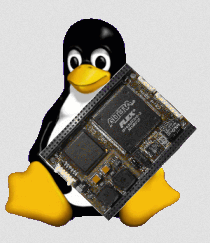
\includegraphics[height=1.5cm]{../images/ThemeEmbedded.png}\\}
              \only<2-6>{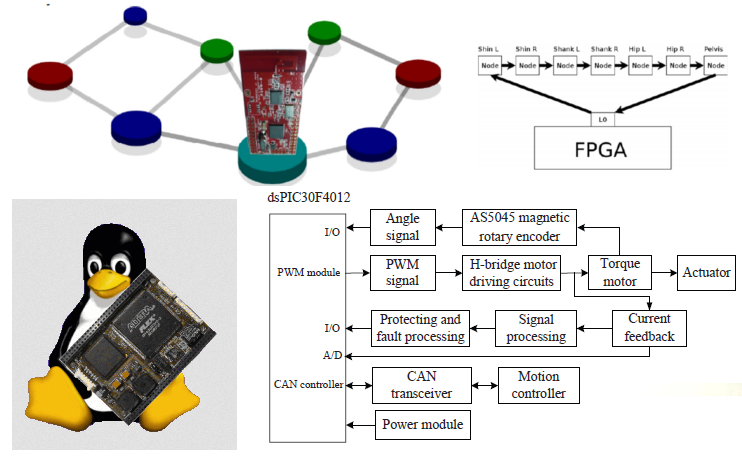
\includegraphics[height=1.5cm]{../images/ShortEmbedded.png}\\}
              \textbf{Sistemas Embebidos}
            \end{beamercolorbox}}
        \end{column}
        \begin{column}{3cm}
          \only<1-2,4-7>{\setbeamercolor{postit}{fg=white,bg=yellow!70!black}}
          \only<3>{\setbeamercolor{postit}{fg=white,bg=yellow}}
          \hyperlink{exp_biomecanica}{
            \begin{beamercolorbox}[sep=0.5em,wd=3cm,rounded=true,center,shadow=true]{postit}
              \only<1-2>{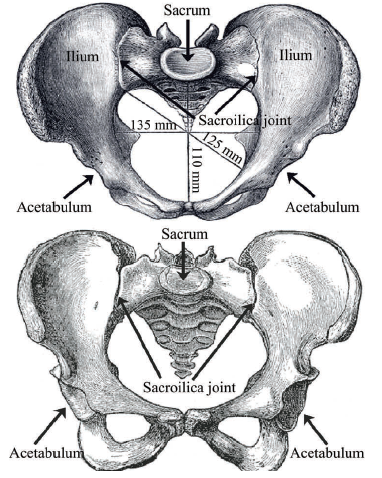
\includegraphics[height=1.5cm]{../images/ThemeBiomechanics.png}\\}
              \only<3-6>{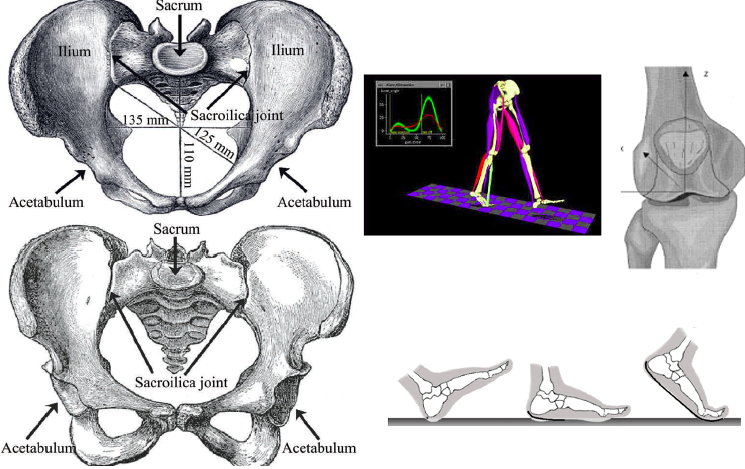
\includegraphics[height=1.5cm]{../images/ShortBiomechanics.png}\\}
              \textbf{Biomec\'anica}
            \end{beamercolorbox}}
        \end{column}
        \begin{column}{3cm}
          \only<1-3,5-7>{\setbeamercolor{postit}{fg=white,bg=blue!50!black}}
          \only<4>{\setbeamercolor{postit}{fg=white,bg=blue}}
          \hyperlink{exp_mecanismos}{
            \begin{beamercolorbox}[sep=0.5em,wd=3cm,rounded=true,center,shadow=true]{postit}
              \only<1-3>{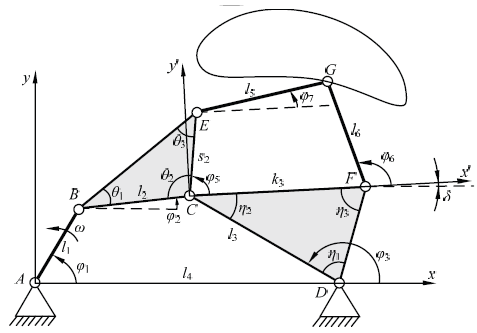
\includegraphics[height=1.5cm]{../images/ThemeMechanisms.png}\\}
              \only<4-6>{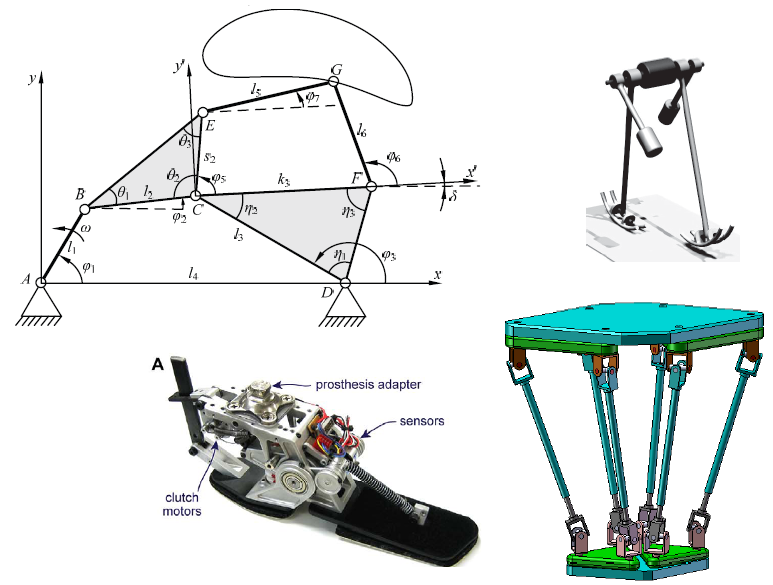
\includegraphics[height=1.5cm]{../images/ShortMechanisms.png}\\}
              \textbf{Modelado y Mecanismos}
            \end{beamercolorbox}}
        \end{column}
      \end{columns}
      \vspace{1.0cm}
      \begin{columns}[c]
        \begin{column}{3cm}
          \only<1-4,6-7>{\setbeamercolor{postit}{fg=white,bg=black}}
          \only<5>{\setbeamercolor{postit}{fg=white,bg=white!50!black}}
          \hyperlink{exp_computacion_flexible}{
            \begin{beamercolorbox}[sep=0.5em,wd=3cm,rounded=true,center,shadow=true]{postit}
              \textbf{C. Flexible y Optimizaci\'on}
              \only<1-4>{\\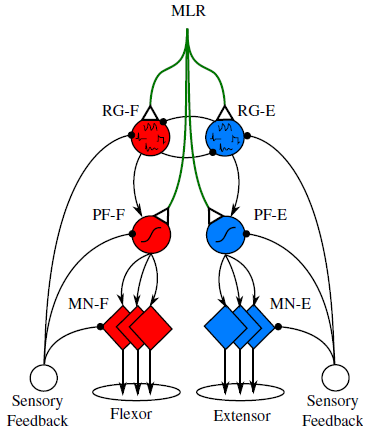
\includegraphics[height=1.5cm]{../images/ThemeSoftComputing.png}}
              \only<5-6>{\\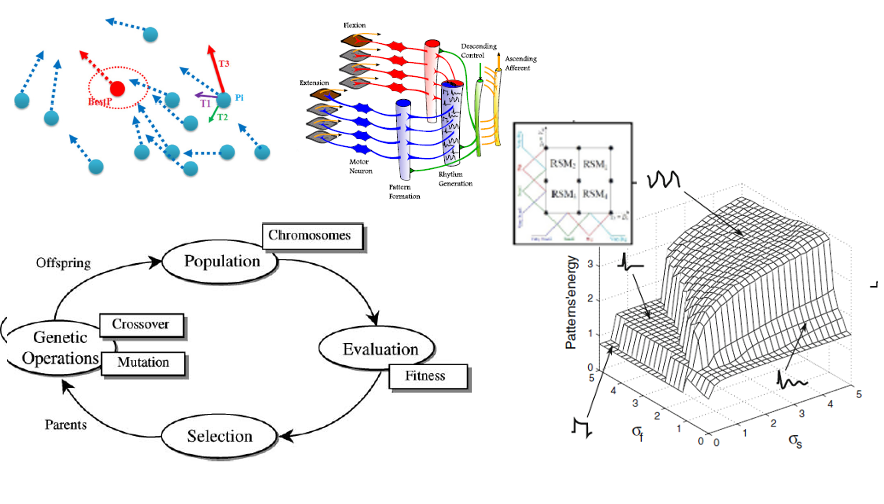
\includegraphics[height=1.5cm]{../images/ShortSoftComputing.png}}
            \end{beamercolorbox}}
        \end{column}
        \begin{column}{3cm}
          \only<1-5,7>{\setbeamercolor{postit}{fg=white,bg=green!50!black}}
          \only<6>{\setbeamercolor{postit}{fg=white,bg=green}}
          \hyperlink{exp_control}{
            \begin{beamercolorbox}[sep=0.5em,wd=3cm,rounded=true,center,shadow=true]{postit}
              \textbf{Control y Sis. Din\'amicos}
              \only<1-5>{\\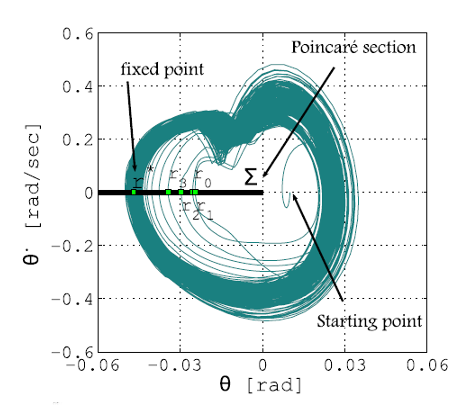
\includegraphics[height=1.5cm]{../images/ThemeControl.png}}
              \only<6-6>{\\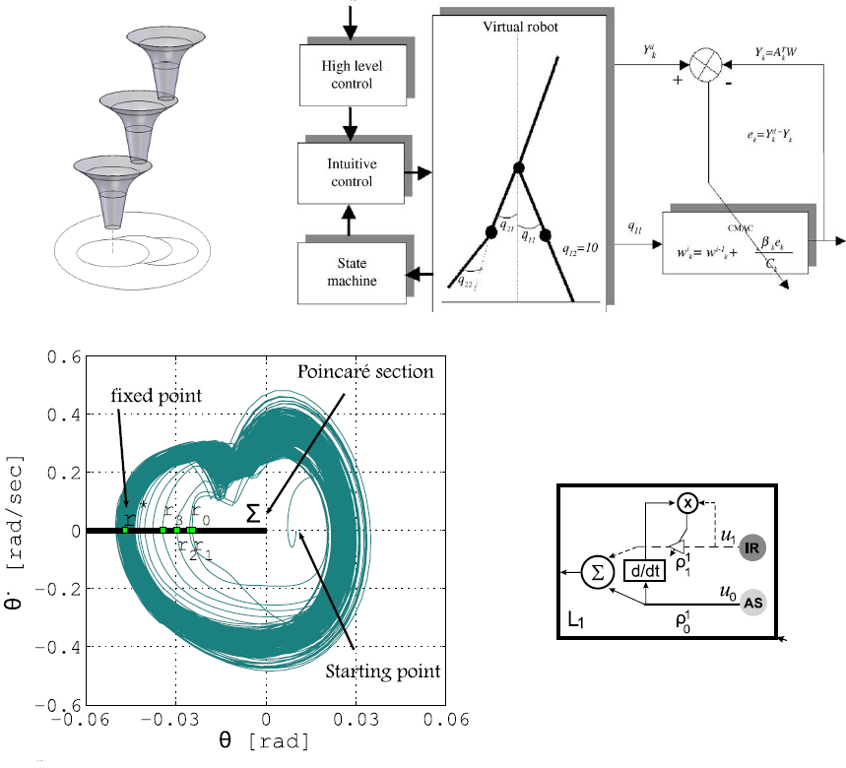
\includegraphics[height=1.45cm]{../images/ShortControl.png}}
            \end{beamercolorbox}}
        \end{column}
      \end{columns}
      \only<1-6>{\vspace{-4.6cm}}
      \only<7>{\vspace{-3.1cm}}
      \hspace{-0.1cm}
      \setbeamercolor{postit}{fg=white,bg=blueun}
      \begin{beamercolorbox}[sep=0.5em,wd=4.0cm,rounded=true,center]{postit}
        \textbf{\Large\textcolor{white}{ROB\'OTICA B\'IPEDA}}
      \end{beamercolorbox}
    }
  \end{center}
\end{frame}